\documentclass{article}

\usepackage{tikz}
\usetikzlibrary{arrows,shapes,backgrounds,patterns,positioning}
\usepackage[latin1]{inputenc}


\begin{document}
  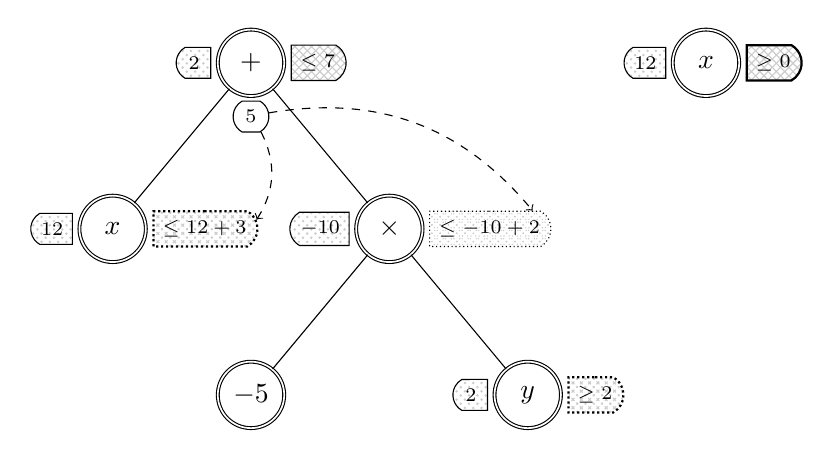
\begin{tikzpicture}[
    label distance = 0.75mm,
    sibling distance = 10em,
    level distance = 6em,
    every label/.style = {rounded rectangle,rounded rectangle arc length=120,
      font=\scriptsize, pattern color=black!20},
    model/.style = {draw,rounded rectangle right arc=none,pattern=crosshatch dots},
    constraint/.style = {draw,rounded rectangle left arc=none,pattern=crosshatch},
    syn/.style = {draw,double,circle,minimum size=2.4em},
    slack/.style = {draw,label distance=0.5mm}
    ]
    \node [syn,label={[model]left:{\(2\)}},
               label={[constraint]right:{\(\le 7\)}},
               label={[slack,name=slack]below:{\(5\)}}] (root) {\(+\)}
      child {node [syn,
             label={[model]left:{\(12\)}},
             label={[constraint,densely dotted,thick,name=const1]right:{\(\le 12+3\)}}] {\(x\)}}
      child {node [syn,
                   label={[model]left:{\(-10\)}},
                   label={[constraint,densely dotted,name=const2]right:{\(\le -10+2\)}}] {\(\times\)}
        child {node [syn]  {\(-5\)}}
        child {node [syn,
                     label={[model]left:{\(2\)}},
                     label={[constraint,densely dotted,thick]right:{\(\ge 2\)}}] {\(y\)}}
    };
    \draw[dashed,->] (slack) edge [bend left] (const1.10);
    \draw[dashed,->] (slack) edge [bend left] ([xshift=-3pt]const2.north east);
    \node [syn,right=14em of root,label={[model]left:{\(12\)}},
    label={[constraint,thick]right:{\(\ge 0\)}}] {\(x\)};
  \end{tikzpicture}
\end{document}
